\setcounter{section}{5}
\setcounter{subsection}{10} % 5.11
\subsection{TCP-Zustandsdiagramm}

\begin{enumerate}[(a)]
    \item Wie kommt der Client in den Zustand {\ttfamily SYN RCVD} bzw. {\ttfamily SYN EMPFANGEN}?

        Der Client kommt nicht in den Zustand {\ttfamily SYN RCVD}. Das ist
        ausschlie{\ss}lich ein Server-Zustand. {\ttfamily SYN RCVD} entsteht,
        wenn ein Server im Zustand {\ttfamily LISTEN} eine {\ttfamily
        SYN}-Nachricht vom Client empf"angt. Siehe Abbildung~\ref{fig:5.11.a}

        \begin{figure}[p]
            \centering
            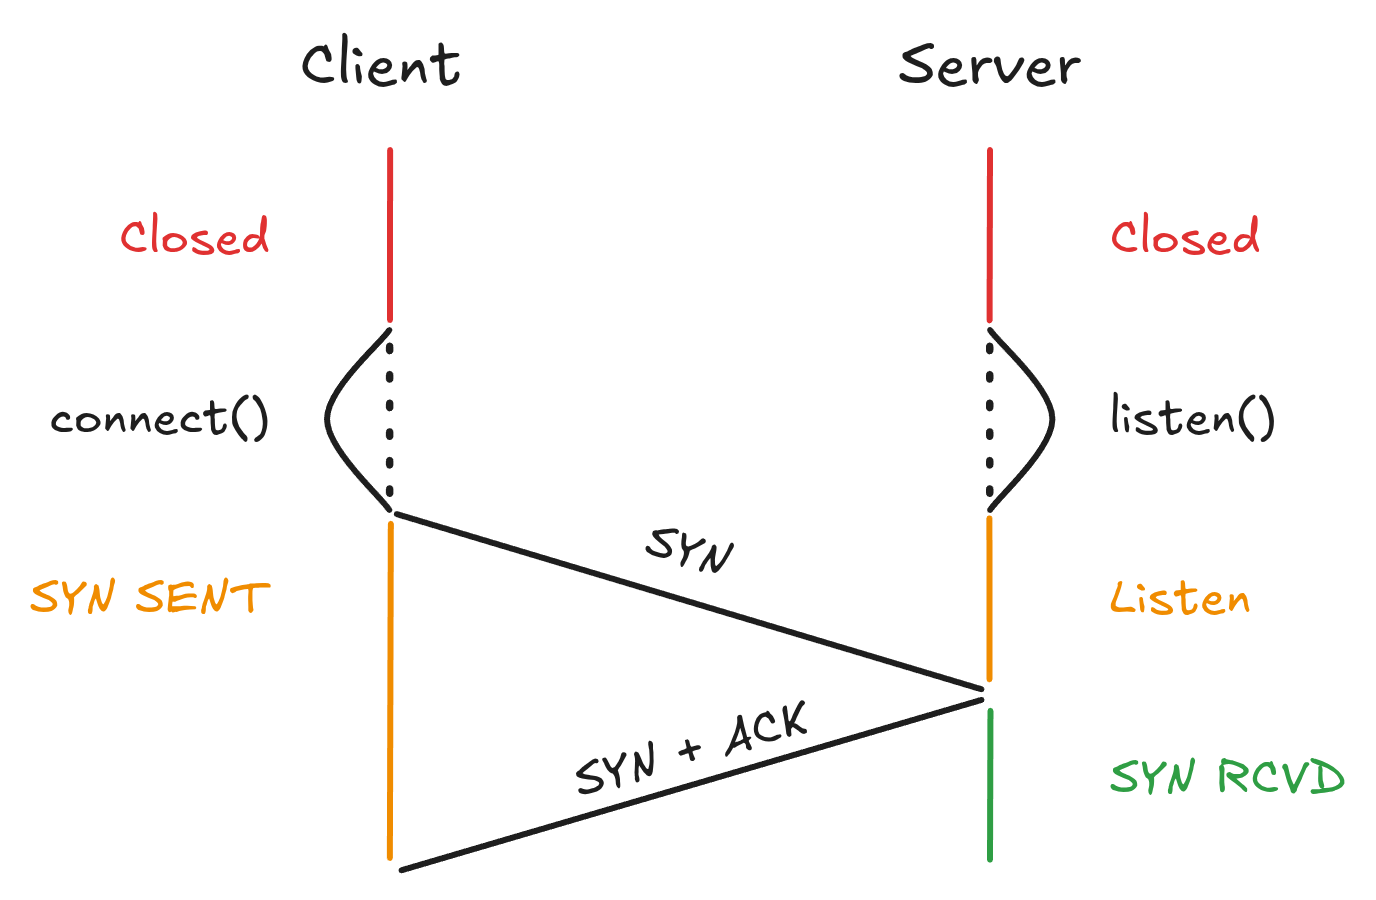
\includegraphics[width=1\textwidth]{./assets/5.11.a.png}
            \caption{}
            \label{fig:5.11.a}
        \end{figure}

        P.S. Unter bestimmten Umständen könnte ein Client auch in den Zustand
        {\ttfamily SYN RCVD} gelangen, wenn er gleichzeitig als Server agiert
        und eingehende Verbindungen akzeptiert. Das tritt zum Beispiel in
        {\ttfamily P2P}-Netzwerken auf, wo beide Teilnehmer sowohl als Client
        als auch als Server fungieren können.

    \item Unter welchen Umständen kommt es zu einem Durchlaufen der Zustände
        {\ttfamily ESTABLISHED}, {\ttfamily FIN WAIT 1}, {\ttfamily CLOSING}
        und {\ttfamily TIME WAIT}?

        Das kann passieren, wenn beide Endpunkte gleichzeitig die Verbindung
        schließen wollen. Siehe Abbildung~\ref{fig:5.11.b}

        \begin{figure}[p]
            \centering
            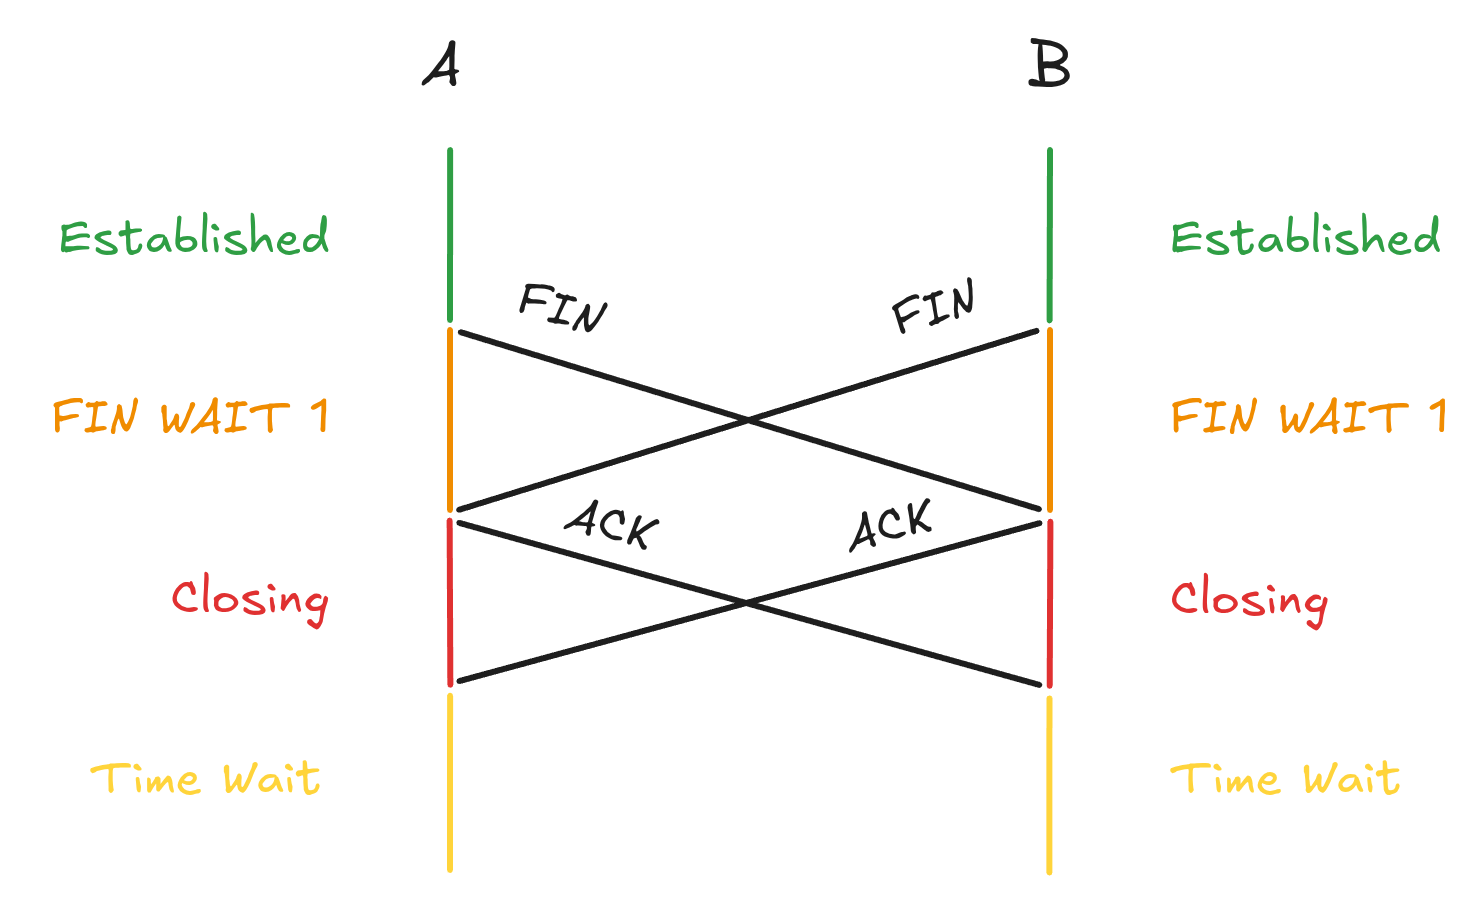
\includegraphics[width=1\textwidth]{./assets/5.11.b.png}
            \caption{}
            \label{fig:5.11.b}
        \end{figure}
\end{enumerate}
